\documentclass[10pt,a4paper]{article}

\usepackage[english]{babel}
\renewcommand*\ttdefault{txtt}
\usepackage[T1]{fontenc}

\usepackage[round,authoryear]{natbib}

\usepackage[hidelinks]{hyperref}

\usepackage{graphicx}
\graphicspath{{./images/}}

\usepackage{listings}
\lstdefinelanguage{scala}{
  morekeywords={abstract,case,catch,class,def,do,else,extends,false,
                final,finally,for,if,implicit,import,match,mixin,new,
                null,object,override,package,private,protected,
                requires,return,sealed,super,this,trait,true,try,
                type,val,var,while,with,yield},
  otherkeywords={=,=>,<-,<\%,<:,>:,\#,@},
  sensitive=true,  
  morecomment=[l]//,
  morecomment=[n]{/*}{*/}, %or [s]
  morestring=[b]",
  morestring=[b]',
  morestring=[b]"""
}
\lstset{
  %frame=tb,
  language=scala,
  %aboveskip=3mm,
  %belowskip=3mm,
  showstringspaces=false,
  numbers=left,
  breaklines=false,
  columns=flexible,
  captionpos=t,
  basicstyle={\footnotesize\ttfamily}
}

\renewcommand\appendix{\par
\setcounter{section}{0}%
\setcounter{subsection}{0}%
\setcounter{table}{0}
\setcounter{figure}{0}
\setcounter{equation}{0}
\gdef\thetable{\Alph{table}}
\gdef\thefigure{\Alph{figure}}
\gdef\theequation{\Alph{section}-\arabic{equation}}
\section*{Appendix}
\gdef\thesection{\Alph{section}}
\setcounter{section}{0}}

\title{Visualizing Project Relations on GitHub}
\author{
    Hendrik van Antwerpen\\{\small\href{mailto:H.vanAntwerpen@student.tudelft.nl}{\nolinkurl{H.vanAntwerpen@student.tudelft.nl}}}
  \and
    Niels van Kaam\\{\small\href{mailto:N.vanKaam@student.tudelft.nl}{\nolinkurl{N.vanKaam@student.tudelft.nl}}}
}
\date{Software Engineering Research Group, EECMS\\Delft University of Technology}

\begin{document}

\maketitle

\begin{abstract}
GitHub has emerged as an interesting object of study for software repository analysis because of the data available through its open API. Visualizing this data can be challenging, because of the lack of knowledge about its structure and because of the size of the dataset. For distributed processing of large data sets functional programming languages and techniques and models like MapReduce have become increasingly popular. In this report we describe a web based system that makes it possible to explore one type of relation in GitHub, the links between projects based on common committers. Users can explore the data by selecting time limits, link degrees and project language. This report describes the implementation of that system in the object-oriented function programming language Scala, using Sawzall style aggregators and other function programming techniques.
\end{abstract}

\section{Introduction}

In the field of software repository mining, GitHub has emerged as an interesting subject of study and tools have emerged to collect and publish the data it publishes \citep{gousios2012ghtorrent}. Making sense of the data and visualizing it in interesting ways is not trivial. Finding interesting correlations and metrics is hard. Interactive software that visualizes aspects of the data while the user can influence constraints like time period or project language allows easy exploration of the data and can be a starting point for more formal analysis.

We present a web based software system that allows a user to explore relations between projects on GitHub. A relation is defined by the existence of a common committer. The user can influence the time period wherein the link must exists, the main programming language of the project and the minimum number of committers before a link is shown.

We identify several challenges in the design of the software:
\begin{itemize}
    \item Providing a general visualization that might reveal interesting properties of the data to the user.
    \item Dealing with the large size of the data that is being processed.
    \item Ensuring responsiveness and reduce waiting times of the software to encourage the user to explore.
\end{itemize}

The software was developed in the context of a functional programming course\footnote{\url{http://swerl.tudelft.nl/bin/view/Main/FunctionalProgrammingCourse}} at the Delft University of Technology. The course focused on functional programming techniques, application of these techniques in more imperative languages and using them for processing large data sets. The report therefore also describes how the functional programming and data processing techniques from the course were applied. The project was implemented using Scala and the code samples will be mostly in that language.

The report is structured as following:
\begin{itemize}
    \item A description of the data and the data processing (section \ref{sec:data}).
    \item A description of a MapReduce implementation in Scala, created to implement the data processing (section \ref{sec:mapreduce}).
    \item A description of the distributed design of the backend, created to improve responsiveness of the software (section \ref{sec:distributed}).
    \item A description of the visualization used in the software (section \ref{sec:visualization}).
    \item Conclusions and ideas for further research and development (section \ref{sec:conclusions}).
\end{itemize}

\section{GitHub data analysis}\label{sec:data}

The data we used was a list of all projects with their main programming language, a list of all users and a list of all commits on GitHub. A commit provides the basic link between a user and a project at a certain time. To give you an impression here are some statistics about the data:

\begin{tabular}{l r}
    \hline
    \#projects & ~600k \\
    \#users & ~400k \\
    \#commits & ~14m \\
    \#(user,project)/week & 3m \\
    \#links & 400k \\
    \hline
\end{tabular}

Some more details on the date can be seen in figures \ref{fig:commits-by-date} (commits over time), \ref{fig:link-degree-hist} (link degree) and \ref{fig:projects-per-user-hist} (projects per user).

\begin{figure}[htb]
    \centering
    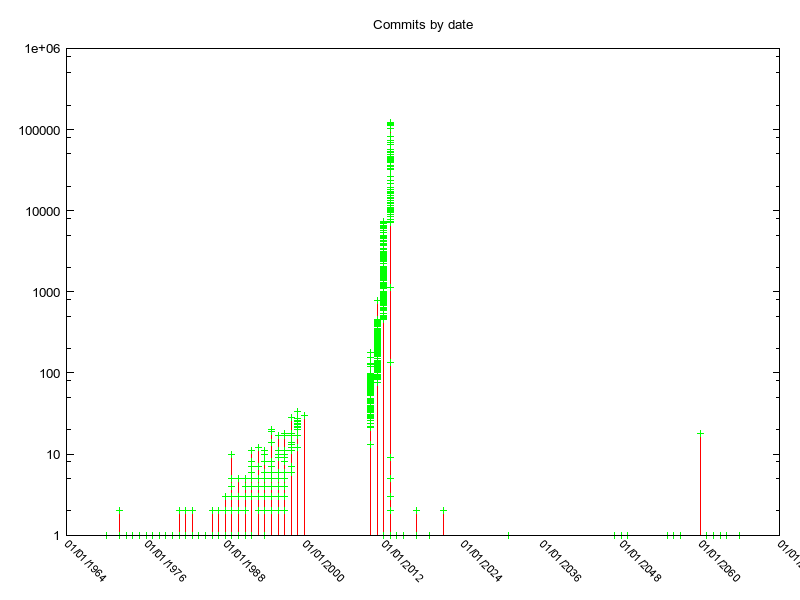
\includegraphics[width=0.75\textwidth]{commits-per-week}
    \caption{Commits by date}
    \label{fig:commits-by-date}
\end{figure}

\begin{figure}[htb]
    \centering
    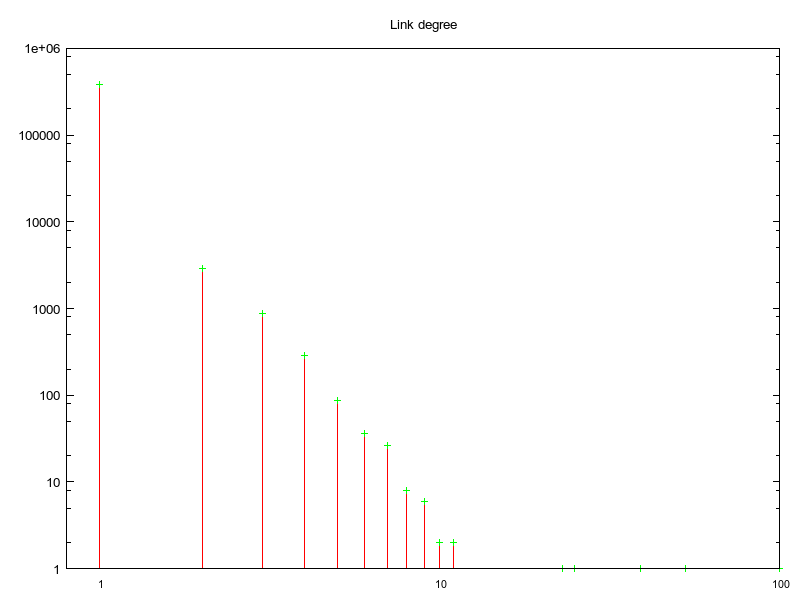
\includegraphics[width=0.75\textwidth]{link-degree-histogram}
    \caption{Link degree histogram}
    \label{fig:link-degree-hist}
\end{figure}

\begin{figure}[htb]
    \centering
    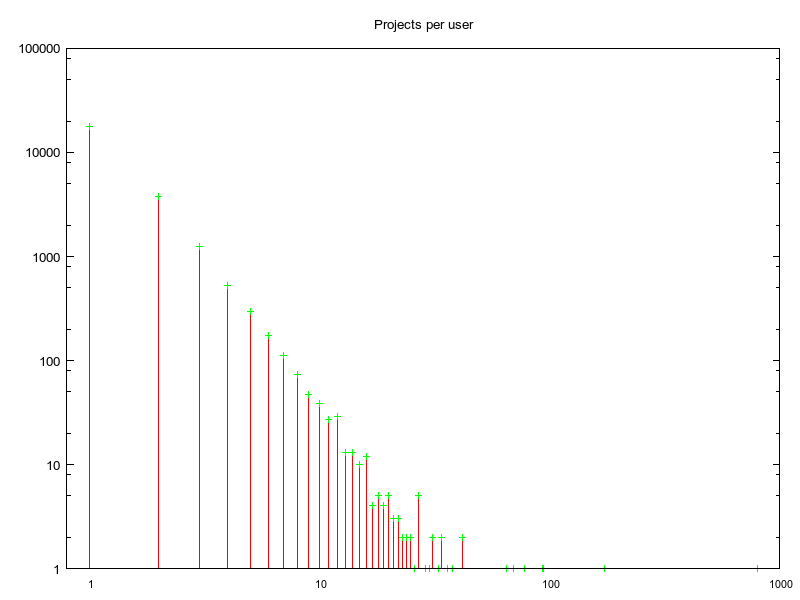
\includegraphics[width=0.75\textwidth]{projects-per-user-histogram}
    \caption{Projects per user histogram}
    \label{fig:projects-per-user-hist}
\end{figure}

We allow the user to vary the following parameters:
\begin{itemize}
    \item Project language (limits projects within one ecosystem).
    \item Time period in which the links are counted.
    \item Minimum degree of a link before it's shown.
\end{itemize}
The desired end result is a list of links between projects, a weight on each link of the amount of common committers and a weight on each project of the amount of connected projects. This last property can identify central projects in the graph.

Processing data can be elegantly expressed as a stream of filter and transform operations. For our purpose they are:
\begin{enumerate}
    \item filter projects for selected language
    \item filter commits and exclude commits outside of the selected time period or not in the filtered project list
    \item create a set of projects per user
    \item per user, create links between all those projects
    \item merge all project links, assigning them weight based on their occurrence
    \item transform the list of links to a format understood by the visualization code
\end{enumerate}

\section{MapReduce with Scala collections}\label{sec:mapreduce}

An increasingly popular model for processing big data sets is MapReduce \citep{dean2008mapreduce}. This model lends itself well for distribution and parallel data processing. One descendant of this model is found in Google's Sawzall \citep{pike2005interpreting}, using aggregators as a key abstraction. In \cite{lammel2008google} a rigorous description of these two models is provided. The Sawzall concept of aggregators is identified as a generalized form of monoids. Their properties allow easy combination of parallel computed partial results, possible in a hierarchical way. Because monoids for common data types like lists, maps and tuples are readily available, developers need think less about the reduction of intermediate results and can focus on the map part of the process.

Sawzall is very liberal in the output it accepts from map functions. The output can be a monoid, a collection of the monoid or an element if the monoid is a collection itself. To capture all these L\"ammel defines aggregators in terms of generalized monoids:
\begin{lstlisting}[language=haskell]
class Monoid m => Aggregator e m | e -> m
  where
    minsert :: e -> m -> m
\end{lstlisting}

To our knowledge no implementation of this approach is available in Scala. Therefore we implemented a version of aggregators for Scala and used those to implement a map-reduce function that integrates seamless with the Scala collection library.

\subsection{Aggregators}

An aggregator is defined by the following trait:
\begin{lstlisting}
trait Aggregator[A,B] {
  def zero: A
  def insert(a: A, b: B): A
}
\end{lstlisting}
Although L\"ammel requires the type \lstinline|A| to be a monoid, we dropped this requirement for reasons that will become clear later. An \lstinline|Aggregator| where \lstinline|A| and \lstinline|B| are the same type behaves the same as a monoid of that type.

We defined the \lstinline[language=haskell]|minsert| function in Scala as \lstinline!a |<| b!. Whenever this operator is used, the compiler infers a fitting Aggregator. All Scala \lstinline|implicit| rules apply, so if no Aggregator is found there's compile time error, if multiple are found the programmer has to specify programmatically which one to use.

Assuming an appending aggregator for \lstinline|List| and a summing one for \lstinline|Int|, we now can do things like the following:
\begin{lstlisting}
val r:Int = i:Int |<| j:Int // sum ints
val r:List[Int] = l:List[Int] |<| m:List[Int] // concat lists
val r:List[Int] = l:List[Int] |<| i:Int // append int element to list
\end{lstlisting}

Combining our aggregators with type inference and the very generic Scala collections library (see \citep{odersky2009fighting} for more details), we were able to provide aggregators for all Scala collections (including parallel ones) by implementing only seven aggregators. For each one of \lstinline|Set|, \lstinline|Seq| and \lstinline|Map|, we implemented an aggregator for monoid behaviour and one for element insertion. Because we don't require our aggregator collection to be a strict monoid, we could make the monoid aggregator very liberal in its accepted input. The collections library defines every collection type to be a subtype of \lstinline|GenTraversableOnce[A]|. Instead of only accepting collections of the same type to be inserted, we can now accept any collection as long as the element type matches. Here are some examples:
\begin{lstlisting}
val r:List[Int] = l:List[Int] |<| s:Set[Int]
val r:TreeMap[Int,Int] = tm:TreeMap[Int,Int] |<| sm:SortedMap[Int,Int]
//val r:Map[Int,Int] = m:Map[Int,Int] |<| l:List[(Int,Int)] // doesn't work?
\end{lstlisting}
The last example is something that is expected to work (\lstinline|Map[K,V] <: Traversable[(K,V)]|, but is somehow not inferred by the compiler. Discussions online suggest that the compiler doesn't consider the complete type hierarchy when inferring, but only a few levels. The seventh aggregator was implemented to handle this special case.

A nice property of monoids is that they can be structurally combined. For example a tuple with two monoid values is itself a monoid. In our aggregator world, we happen to have similar properties. Aggregators for \lstinline|TupleN| and \lstinline|Map| where implemented to require their tuple values and map value to be aggregators themselves. The fact that we only have aggregators and don't differentiate between monoid append and element insertion really pays of here. When creating deep structures, on every level we have the choice to insert either a value or a collection. Some examples should show the flexibility this gives us:
\begin{lstlisting}
// inserted tuples contain collections or elements. values are independent
val r:(Set[Int],Set[String]) = t1:(Set[Int],Set[String]) |<| t2:(Set[Int],Set[String])
val r:(Set[Int],Set[String]) = t1:(Set[Int],Set[String]) |<| t2:(Int,String)
val r:(Set[Int],Set[String]) = t1:(Set[Int],Set[String]) |<| t2:(Set[Int],String)

// three level deep structures
val m:Map[Int,Set[String]] = Map[Int,Set[String]] |<| Map[Int,Set[String]]
val m:Map[Int,Set[String]] = Map[Int,Set[String]] |<| Map[Int,String]
val m:Map[Int,Set[String]] = Map[Int,Set[String]] |<| (Int,Set[String])
val m:Map[Int,Set[String]] = Map[Int,Set[String]] |<| (Int,String)
\end{lstlisting}

Our design allows a lot of freedom in the shape of the elements inserted into a collection. What type of elements can be inserted is dictated by the defined aggregators and fully inferred by the compiler. The aggregators for the Scala collections are very generic and in most cases the developer doesn't have to care about how to merge collections. For opaque values aggregators are implemented for string concatenation and integer summing, but others are very easy to implement; one implicit function and an implementation of the \lstinline|Aggregator| trait is enough.

\subsection{MapReduce}

Using the aggregators we now have, a map-reduce library was implemented. We wanted the map-reduce functionality to be as easy to use as the standard collection functions, like \lstinline|map| or \lstinline|filter|. To a high degree this can be achieved by enriching libraries, a process similar to defining type classes in Haskell (see \cite{odersky2006pimp} for details).

Using again the generic design of the collections library and type inference allows us to write map-reduce by only specifying the expected result type. A word count example similar to one L\"ammel gives is:
\begin{lstlisting}
val docs: List[String]
def wordcount(doc: String): List[(String,Int)] = doc.split(" ").toList.map( w => (w,1) )
val wc = docs.mapReduce[Map[String,Int]]( wordcount )
// wc has type Map[String,Int] here
\end{lstlisting}

The performance of our map-reduce in the same order and range as hand written code using e.g. \lstinline|foldLeft|. Most of the work is done through inference by the compiler. At runtime the aggregators use folds and collection operations just as you would in handwritten code. There a little overhead of some function calls, but all the reduction details are abstracted away, resulting in less repetition and simpler data transformation functions.

With this result we can write our processing steps from section \ref{sec:data} in Scala. You can see how they mix with the existing collection library functions.
\begin{lstlisting}
val commits: List[Commit] = ...
def projectsToPairs(ps: List[Project]): List[(Project,Project)] = ...
val linkMap = 
  commits.filter( c => c.timestamp >= from && c.timestamp <= until  )
          .mapReduce[Map[User,Set[Project]]]( c => (c.user,c.project) )
          .values
          .mapReduce[Map[(Project,Project),Int]](projectsToParis)
          .filter( _._2 >= minDegree )
\end{lstlisting}

It is possible that multiple aggregators for the same type exist, for example a sum and a product on numbers. In such a case it is very easy to specify which one to use. Here is a small example:
\begin{lstlisting}
def SumMonoid: Aggregator[Int,Int] = ...
def ProductMonoid: Aggregator[Int,Int] = ...

val words: List[String] = ...
val sumOfWordLengths = words.mapReduce( w => w.size )(SumMonoid)
val prodOfWordLengths = words.mapReduce( w => w.size )(ProductMonoid)
\end{lstlisting}
As you can see the result type is not required, because it is inferred from the aggregator.

One aspect of the Sawzall model we described in the beginning is not addressed yet. The possibility to insert a collection. This case is handled by the \lstinline|flatMapReduce| function, which is the map-reduce version of \lstinline|flatMap|. This does nothing more then iterating over a \lstinline|Traversable| and inserting every element individually. Because every Scala collection is a \lstinline|Traversable| of its element type, reductions of collection monoids can be written both with \lstinline|mapReduce| as with \lstinline|flatMapReduce|. The implementation in the former could be more efficient, taking the more specific type into account.

\section{Distributed data-processing with Akka}\label{sec:distributed}

\begin{itemize}
    \item What did we want to address
    \item How did we design the actors, where was the caching, where which processing steps
    \item What was the performance (did we speed up response time?)
    \item A design diagram
\end{itemize}

\section{Visualization in the browser with D3}\label{sec:visualization}

\begin{itemize}
    \item What did we want to show?
    \item How did we implement it (D3, what graph parameters)
    \item How did we emphasize characteristics (e.g. central projects)
    \item An example result
\end{itemize}

\section{Conclusions and further research}\label{sec:conclusions}

\begin{itemize}
    \item Did it work
    \item Is it responsive?
    \item Did we show interesting things
    \item What more interesting things could fit in this framework?
\end{itemize}

We believe the given approach can be easily adapted to include other parameters or show other relations in the data.

\begin{itemize}
    \item Optimization by only considering weeks
\end{itemize}

\bibliographystyle{abbrvnat}
\bibliography{github-relations-viz}

\appendix

\section{Scala collection Aggregator example}

\end{document}